\chapter{Search for Standard Model $\PH \to \Pgt\Pgt$}
\label{chap:httSM}

As described in chapter \ref{chap:theory}, the Higgs boson is the final missing 
piece of the Standard Model of particle physics. In order to complete the SM, 
this Higgs boson should have all the predicted properties of the Standard Model
Higgs, including decaying to tau leptons at the predicted rate. This
chapter describes the search for the Higgs boson of the Standard Model 
decaying into two tau leptons.

This chapter outlines the "legacy" result from run 1 of the LHC, including the
full dataset collected in 2011 and 2012 by CMS. This corresponds to an
integrated luminosity of 4.9 fb$^{-1}$ at a centre of mass energy of 7 TeV and
19.7 fb$^{-1}$ at 8 TeV. The results in this chapter are parts of a publication 
in the Journal of High Energy Physics \cite{}. The material in this chapter is
particularly focussed towards the parts of the analysis which included the work
of the author.

\section{Event Selection}

\section{Backgrounds}

\section{Data/MC Correction Factors}

Whilst data-driven methods are used wherever possible, MC is still
relied on in predicting expected shapes and yields of signal and backgrounds in
each channel and category. As such is it important that the MC is corrected for
any effects which are not well modeled. In part this is achieved by measuring
the efficiencies of the different parts of the event selections in both data and
MC, and deriving a scale factor which is the ratio of these efficiencies and is
applied to the MC as a correction.

Such scale factors can be derived to account for differences in the ID, isolation and trigger
efficiences for the light leptons of the e$\tau_{h}$ and $\mu\tau_{h}$ channels.
This is done using a ``tag and probe" method.
The tag and probe method makes use of a well known and measured resonance decaying
into a light lepton pair, in this case
the Z, with the idea that a pair of either electrons or muons is
reconstructed in which one
is the `tag' and one is the `probe'. The tag is constrained by a very tight
selection so that it is known with near certainty to be a real electron/muon.
The probe is subject to a looser selection, but only tag/probe pairs with a
combined invariant mass close to the Z mass are used. Thus, given that the tag
is subject to a tight selection and the mass of the pair is consistent with
products of a Z, it is almost definite that the probe is indeed a real
electron/muon also. Then the probe can be subjected to further cuts or
constraints to measure the efficiency of such a selection to select real
leptons.

The invariant mass distributions of the tag and probe events are used to extract
the different
selection efficiencies. A simultaneous fit of the mass shapes is performed, and
the ratio of the integral of the fitted Z signal in the pass and fail
distributions is used to extract the efficiency. ???To account for any background
to the signal from real Z events, signal and background are fitted for
separately.??? not sure what this background is

The electron/muon ID efficiency is measured with a reconstructed
electron/muon as the probe. The electron/muon isolation efficiency is measured
with a probe which already fulfills the full ID selection criteria. 

The efficiencies for combined ID and isolation are shown in Figures
\ref{fig:electronIdIso} and \ref{fig:muonIdIso}, measured in the complete 2012
dataset and PU weighted MC, as a function of the lepton $\eta$ and p$_{\rm{T}}$.
The scale factor which is used in the analysis is given by the ratio of the
measured efficiency in data (black) and MC (red), and is evaluated separately in
selected p$_{\rm{T}}$ and $\eta$ bins.

\begin{figure}[h!]
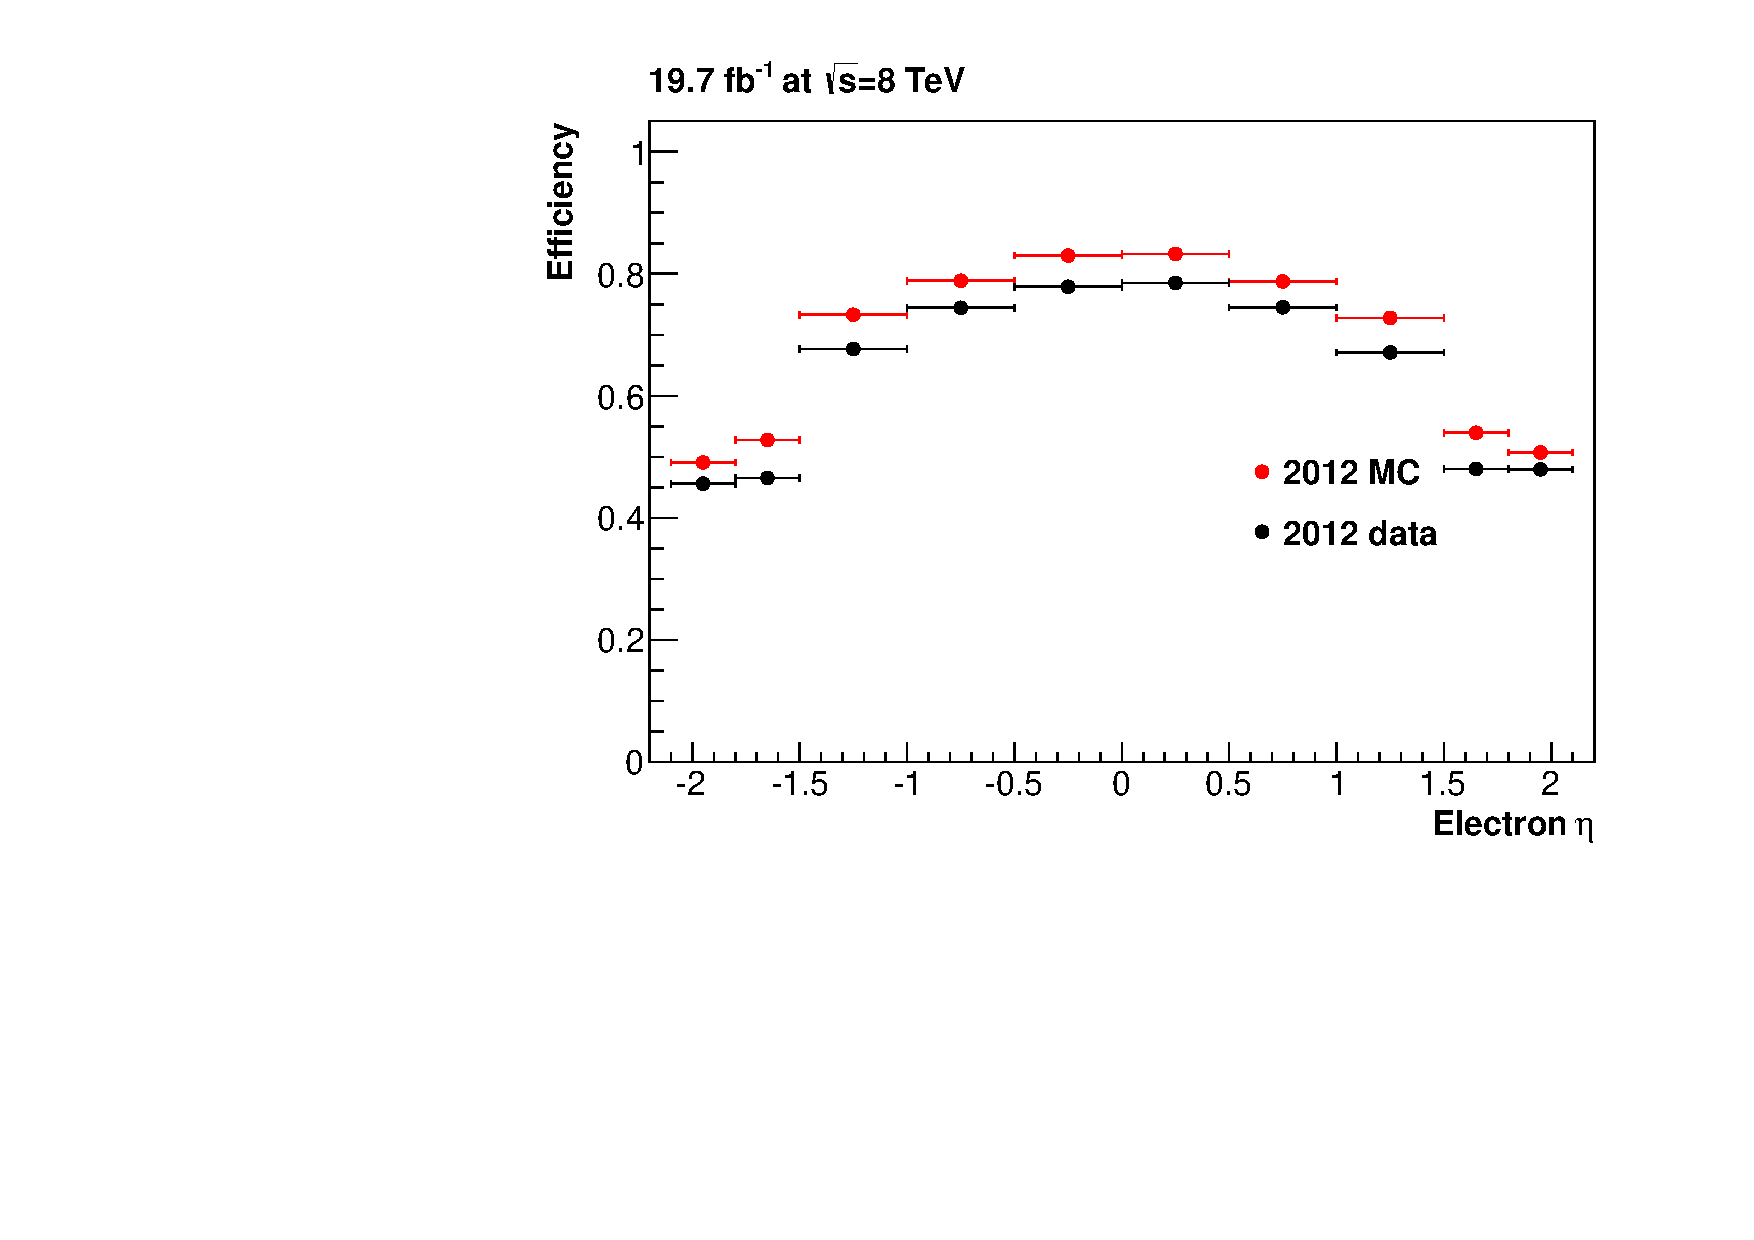
\includegraphics[width=0.5\textwidth]{plots/TagAndProbe/ElectronIdIsoEta2012DatavsMC.pdf}
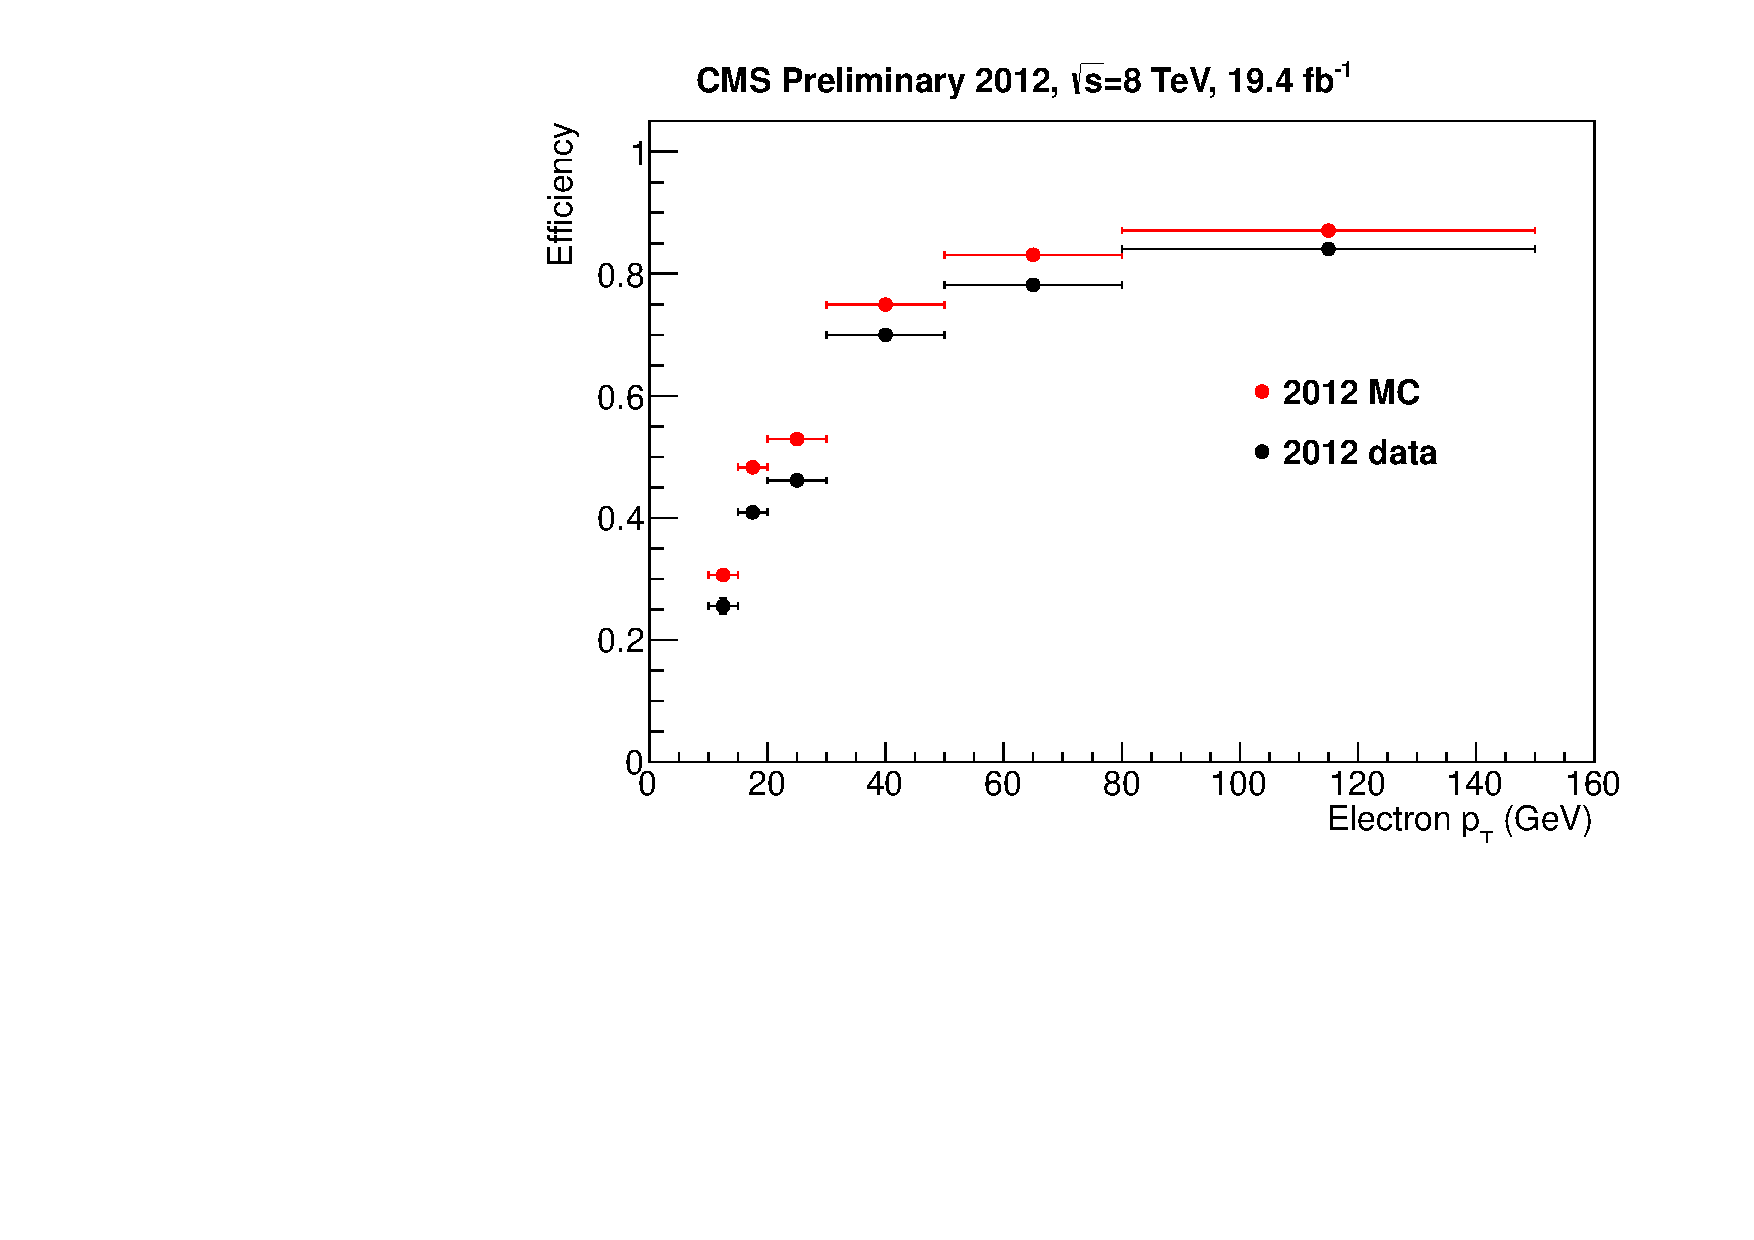
\includegraphics[width=0.5\textwidth]{plots/TagAndProbe/ElectronIdIsoPT2012DatavsMC.pdf}
\caption{Combined electron ID and isolation efficiency in data and MC as a
function of (left) $\eta$ and (right) p$_{\rm{T}}$}
\label{fig:electronIdIso}
\end{figure}

\begin{figure}[h!]
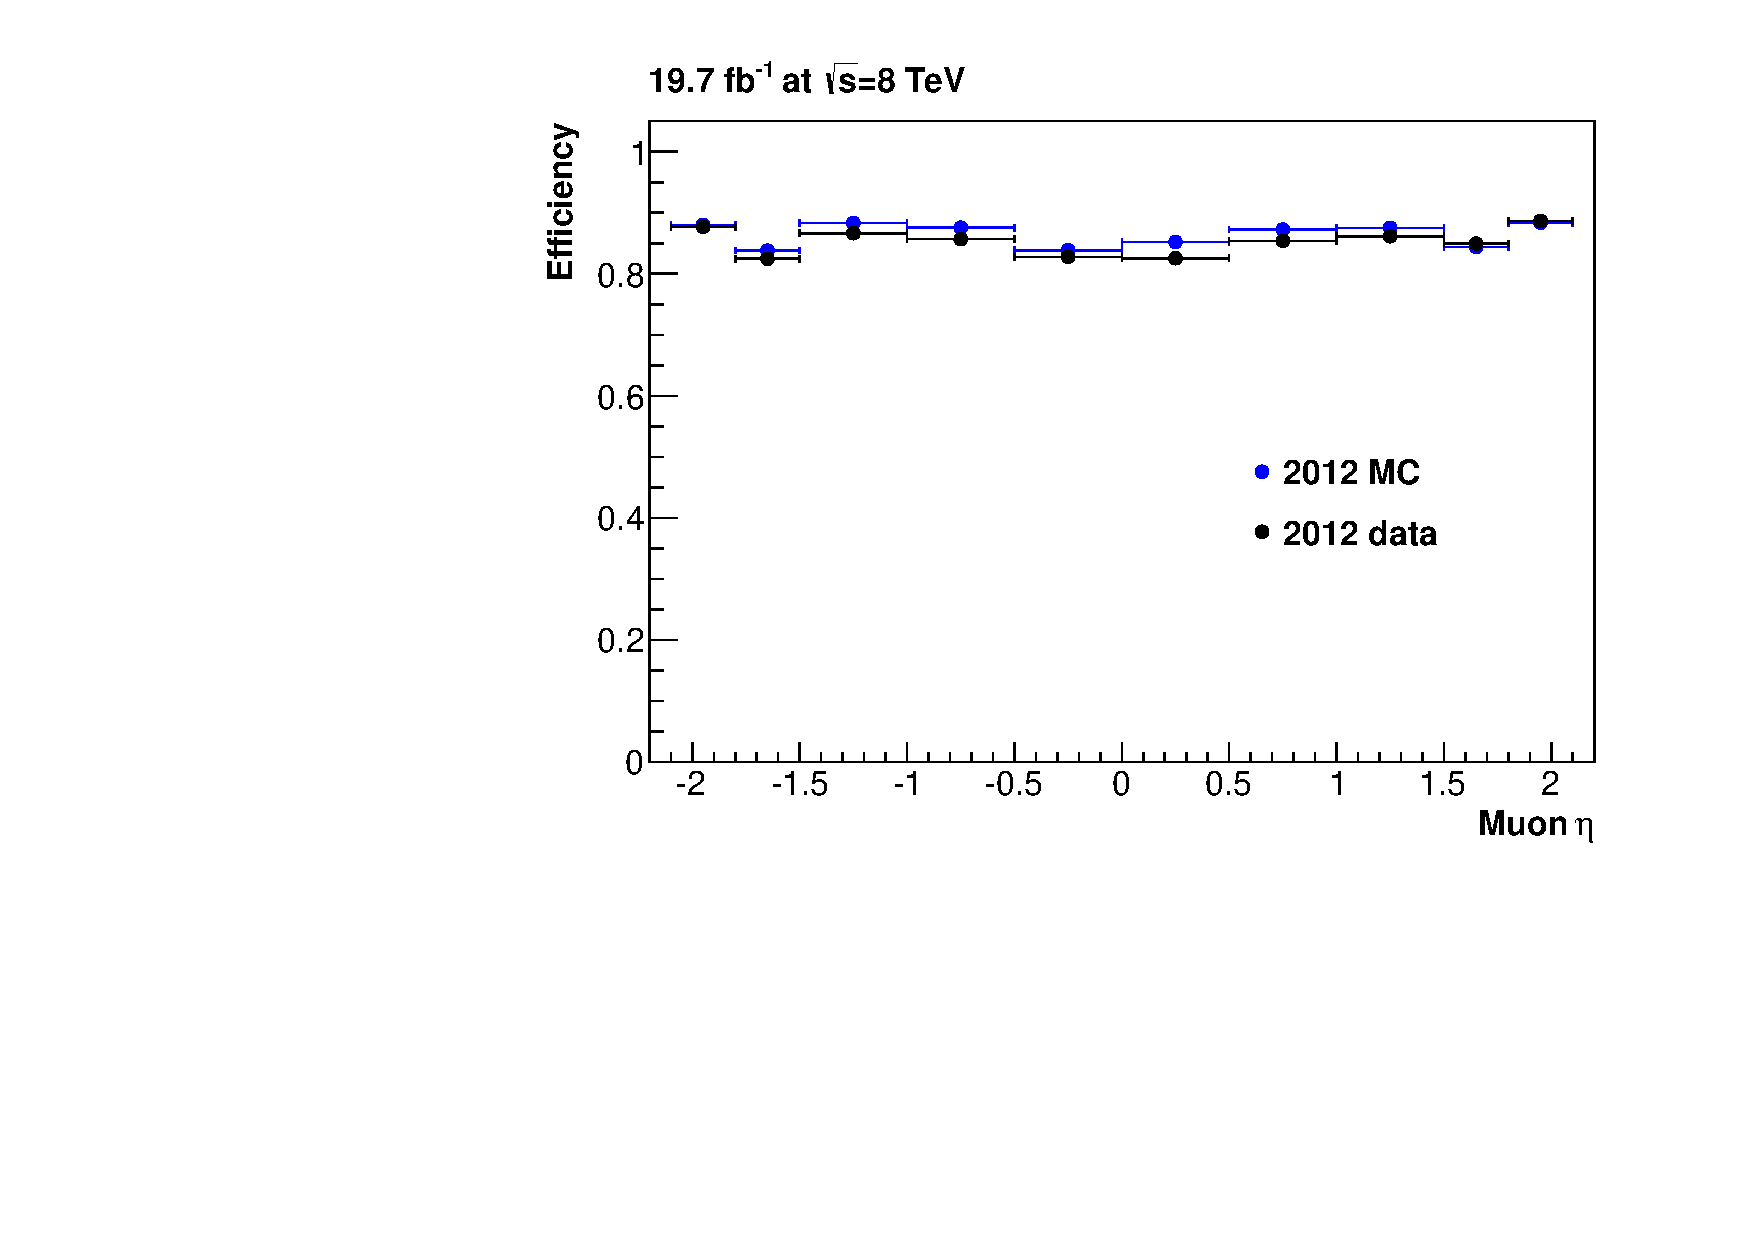
\includegraphics[width=0.5\textwidth]{plots/TagAndProbe/MuonIdIsoEta2012DatavsMC.pdf}
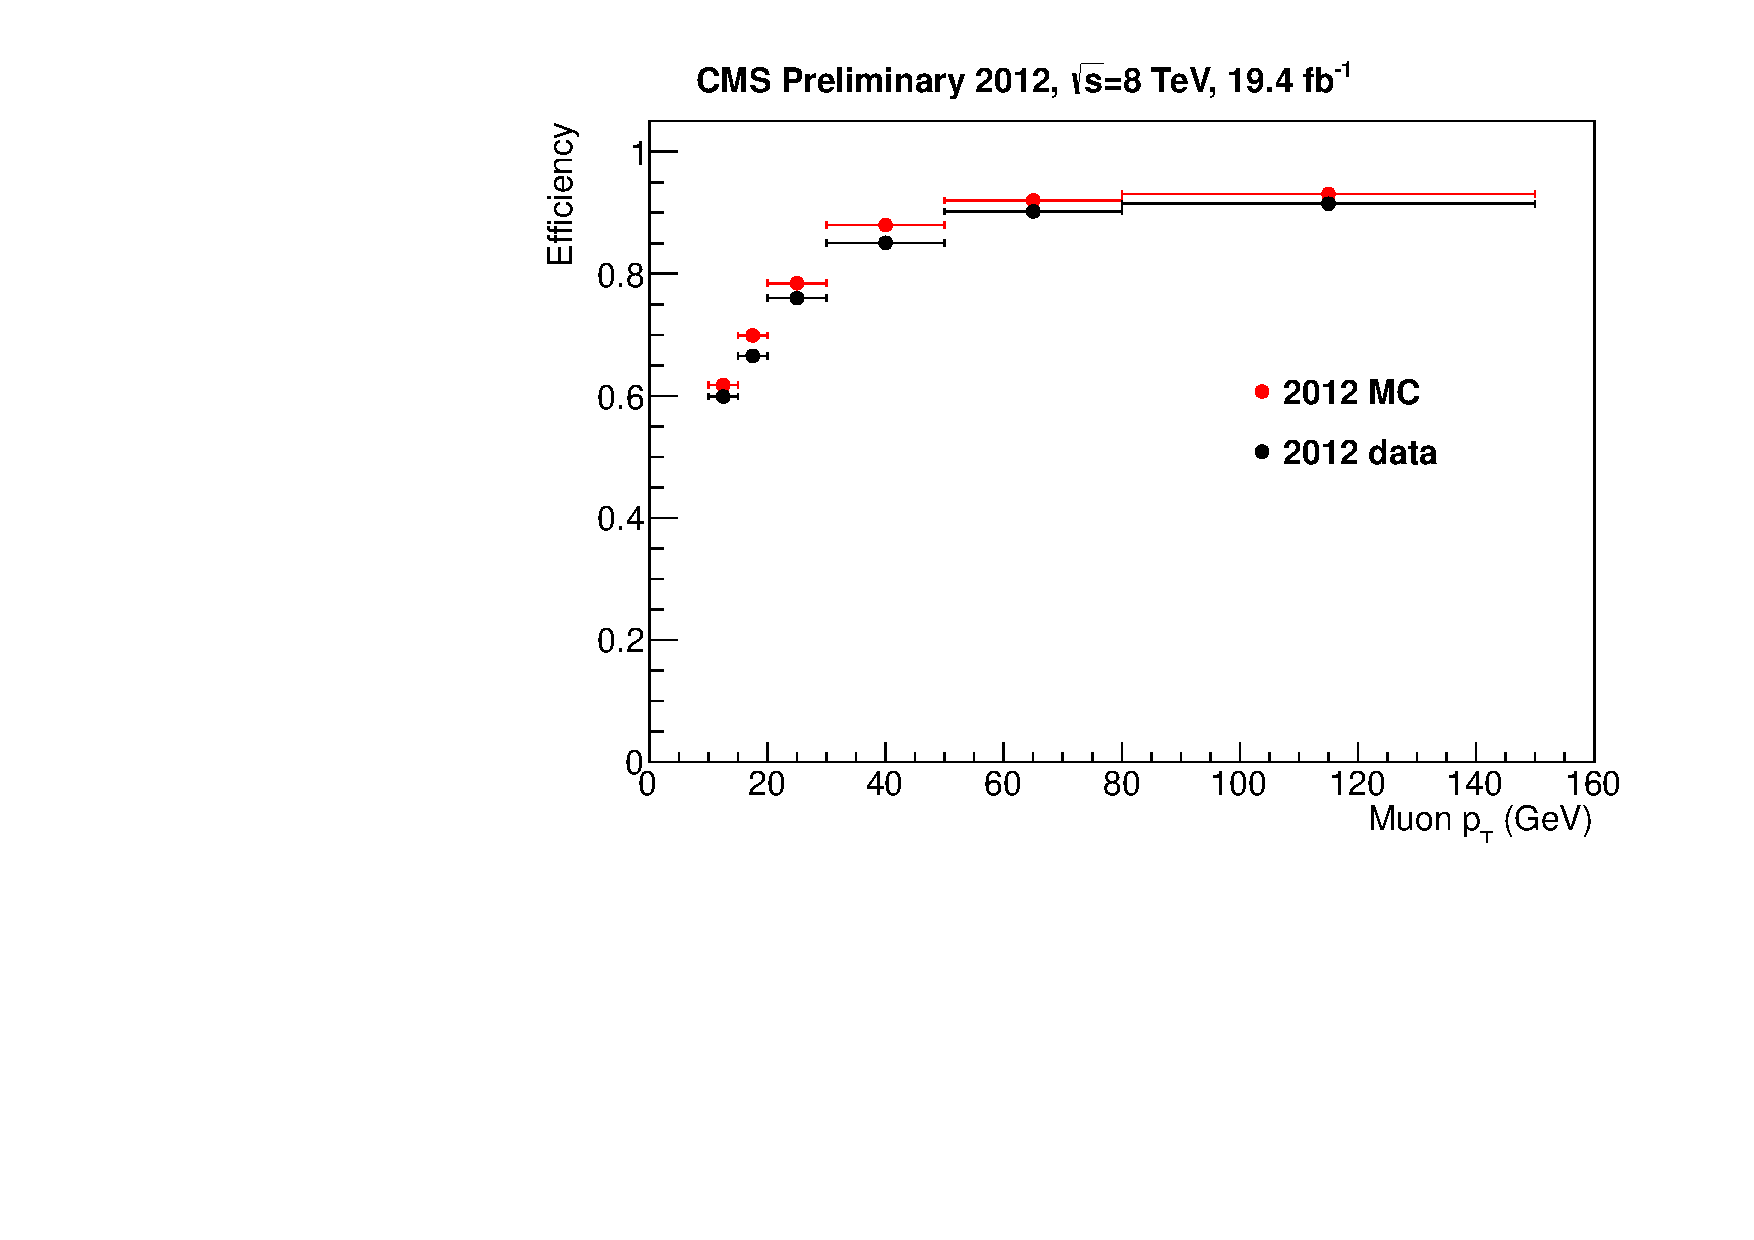
\includegraphics[width=0.5\textwidth]{plots/TagAndProbe/MuonIdIsoPT2012DatavsMC.pdf}
\caption{Combined muon ID and isolation efficiency in data and MC as a function
of (left) $\eta$ and (right) p$_{\rm{T}}$}
\label{fig:muonIdIso}
\end{figure}

\noindent The same method can be used to measure the efficiencies of the trigger
in data and MC. In this case a probe is used which has already passed both ID
and isolation, and the passing probe condition is that the lepton is responsible
for firing the lepton leg of the lepton+tau trigger. Figures
\ref{fig:electrontrg} and \ref{fig:muontrg} show the trigger efficiency as a
function of p$_{\rm{T}}$ measured in both 2012 data and MC. For the
electrons, the trigger is measured separately in the barrel and endcap
regions, which correspond to $|\eta| < 1.479$ and $|\eta| > 1.479$
respectively. For the muons, the trigger is measured in 3 regions, corresponding
to .

\begin{figure}[h!]
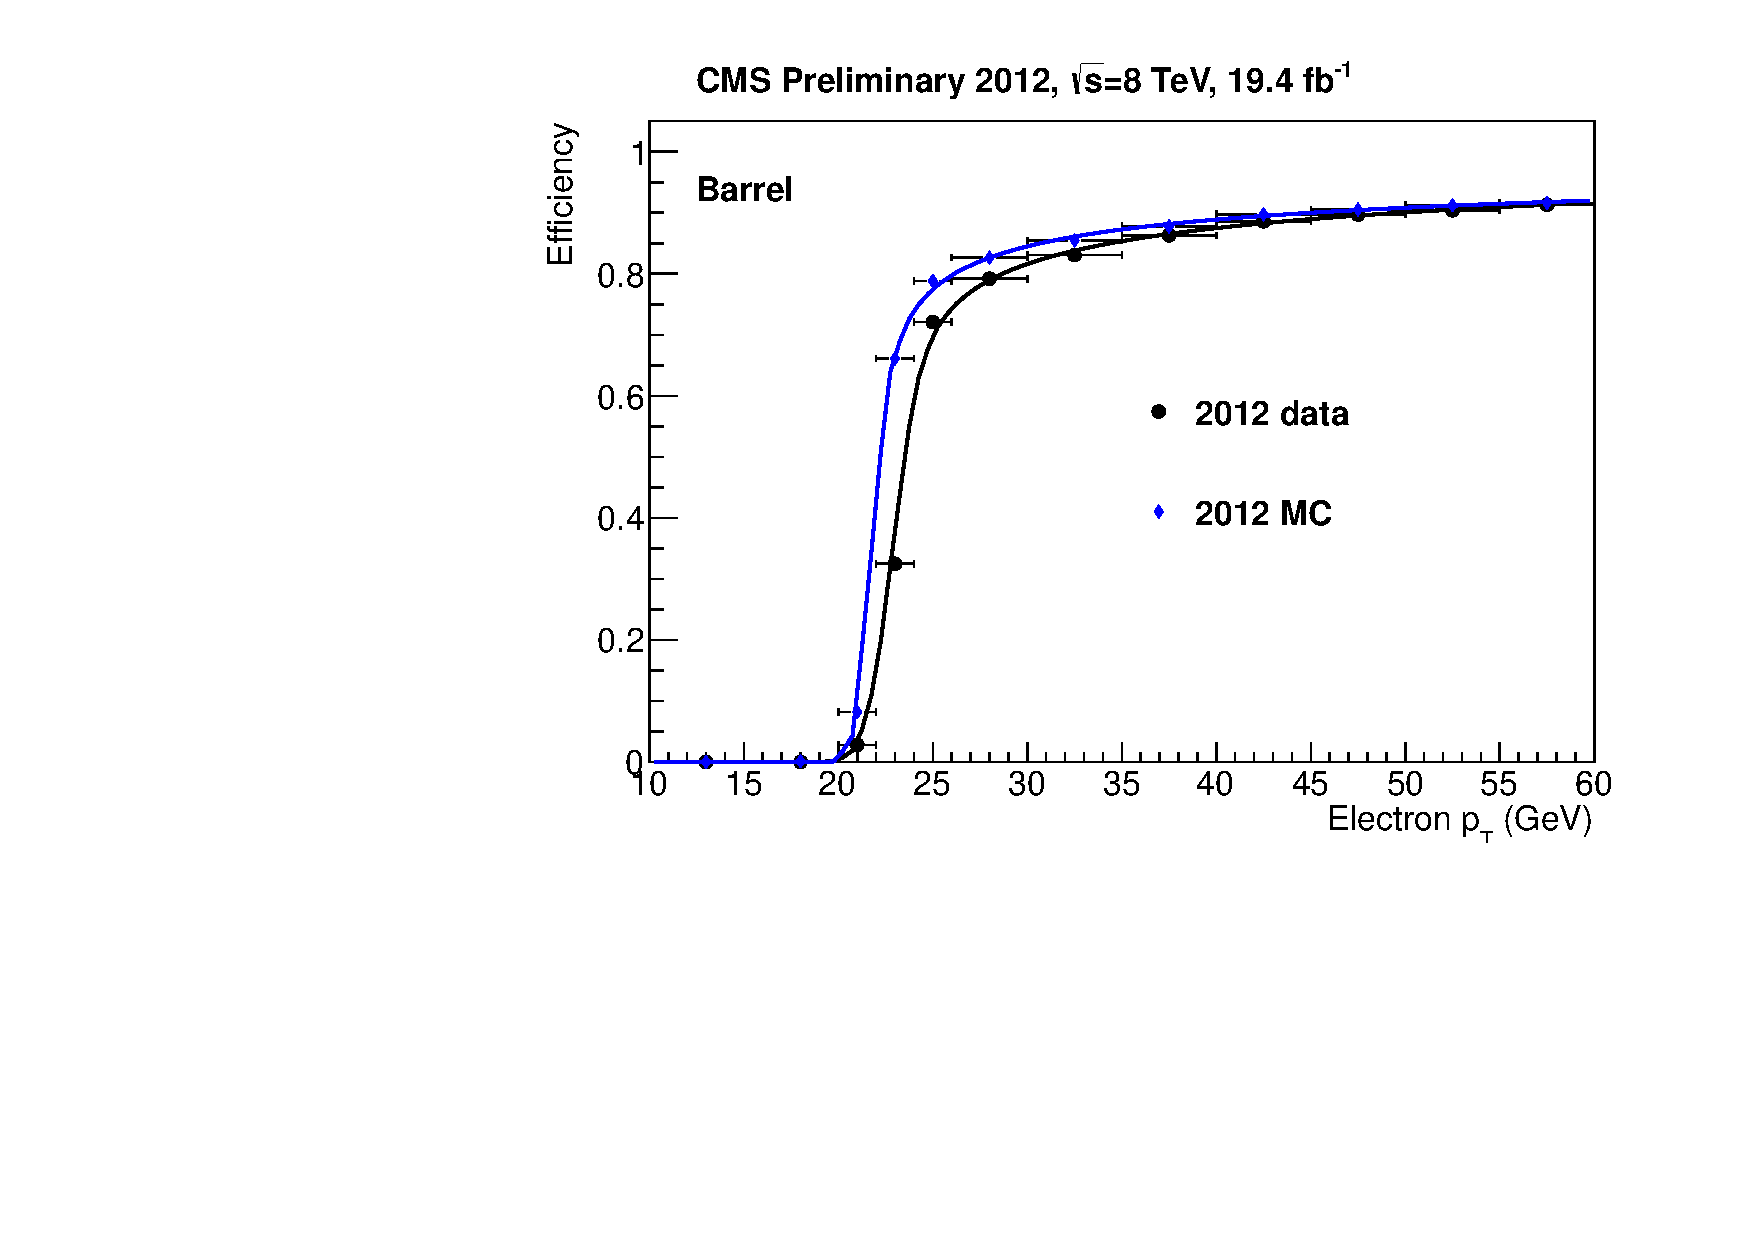
\includegraphics[width=0.5\textwidth]{plots/TagAndProbe/ElectronBarrel2012DatavsMC.pdf}
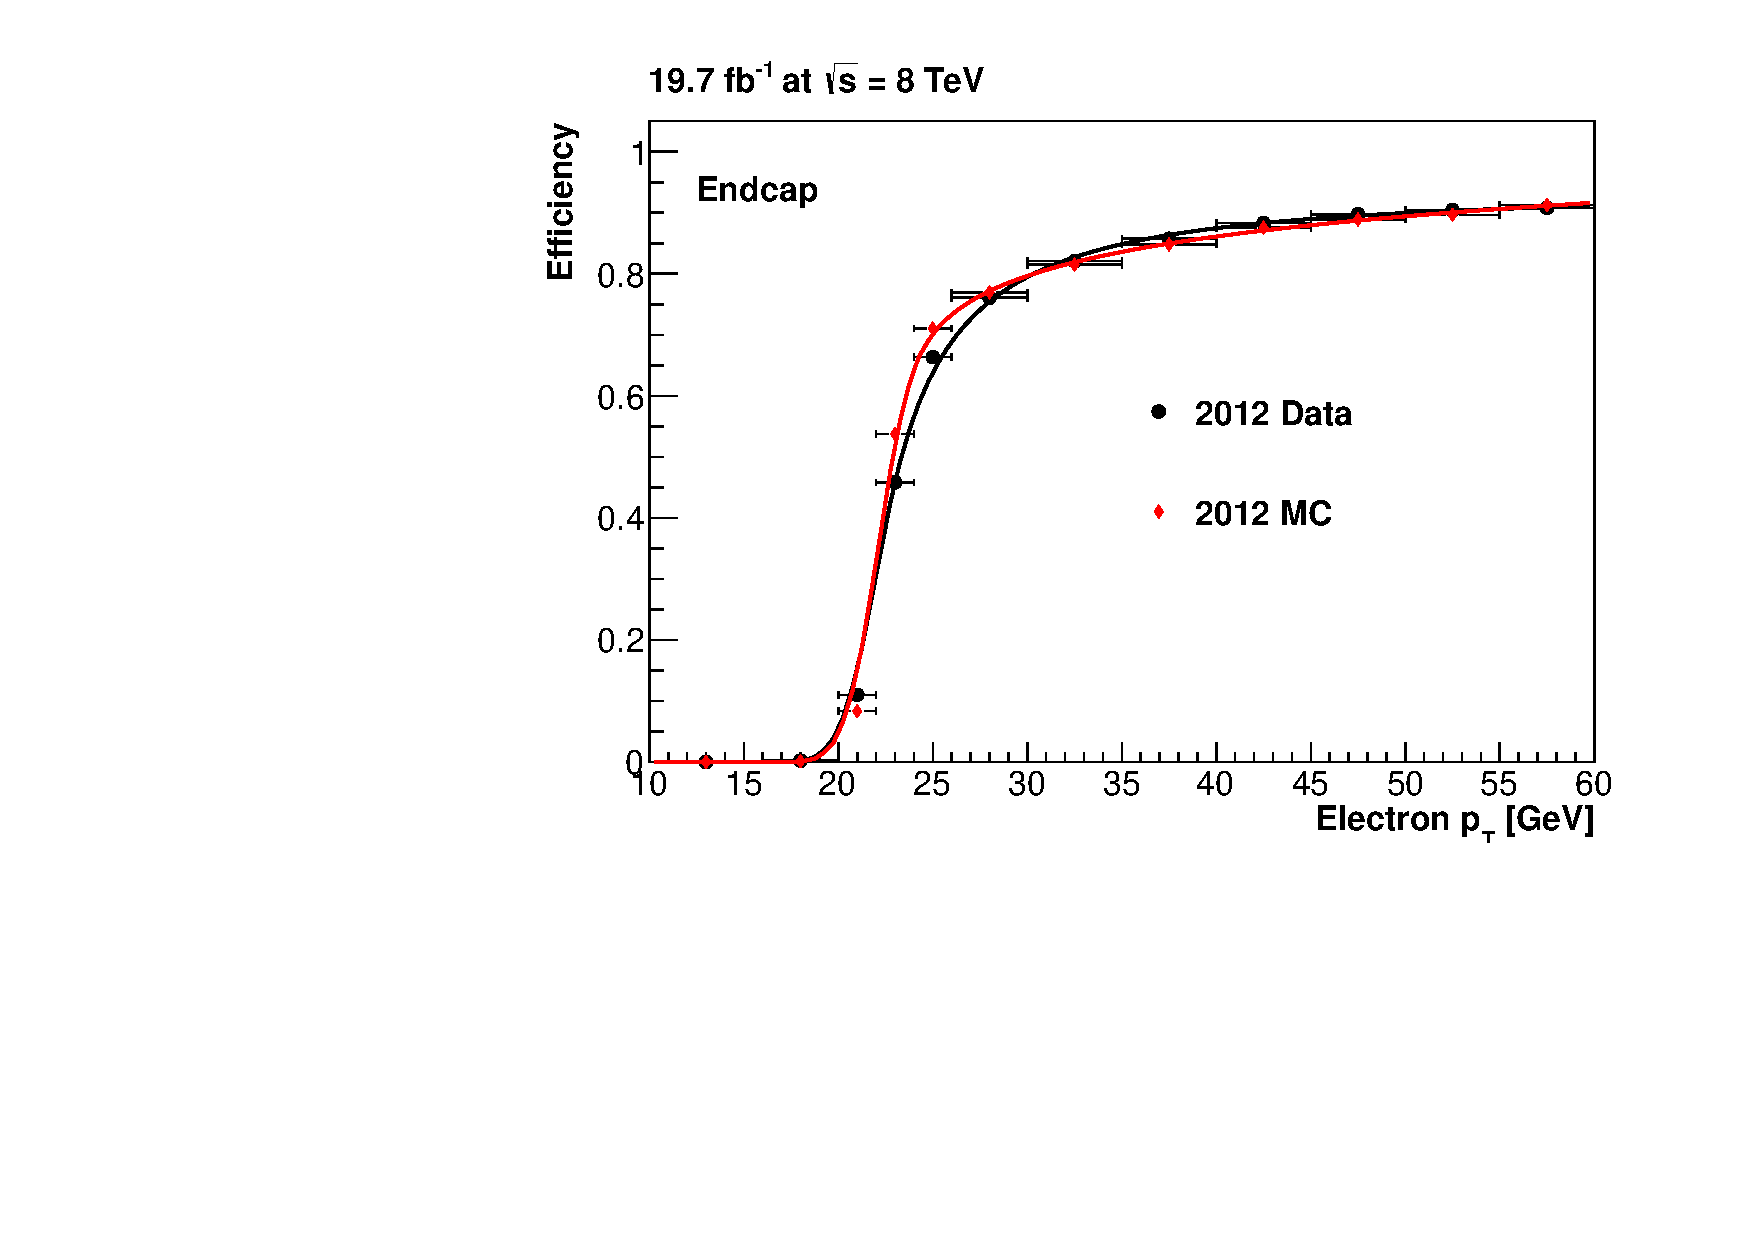
\includegraphics[width=0.5\textwidth]{plots/TagAndProbe/ElectronEndcap2012DatavsMC.pdf}
\caption{Trigger efficiency as a function of electron p$_{\rm{T}}$ measured
in 2012 data and MC in the (left) barrel and (right) endcaps.}
\label{fig:electrontrg}
\end{figure}

\begin{figure}[h!]
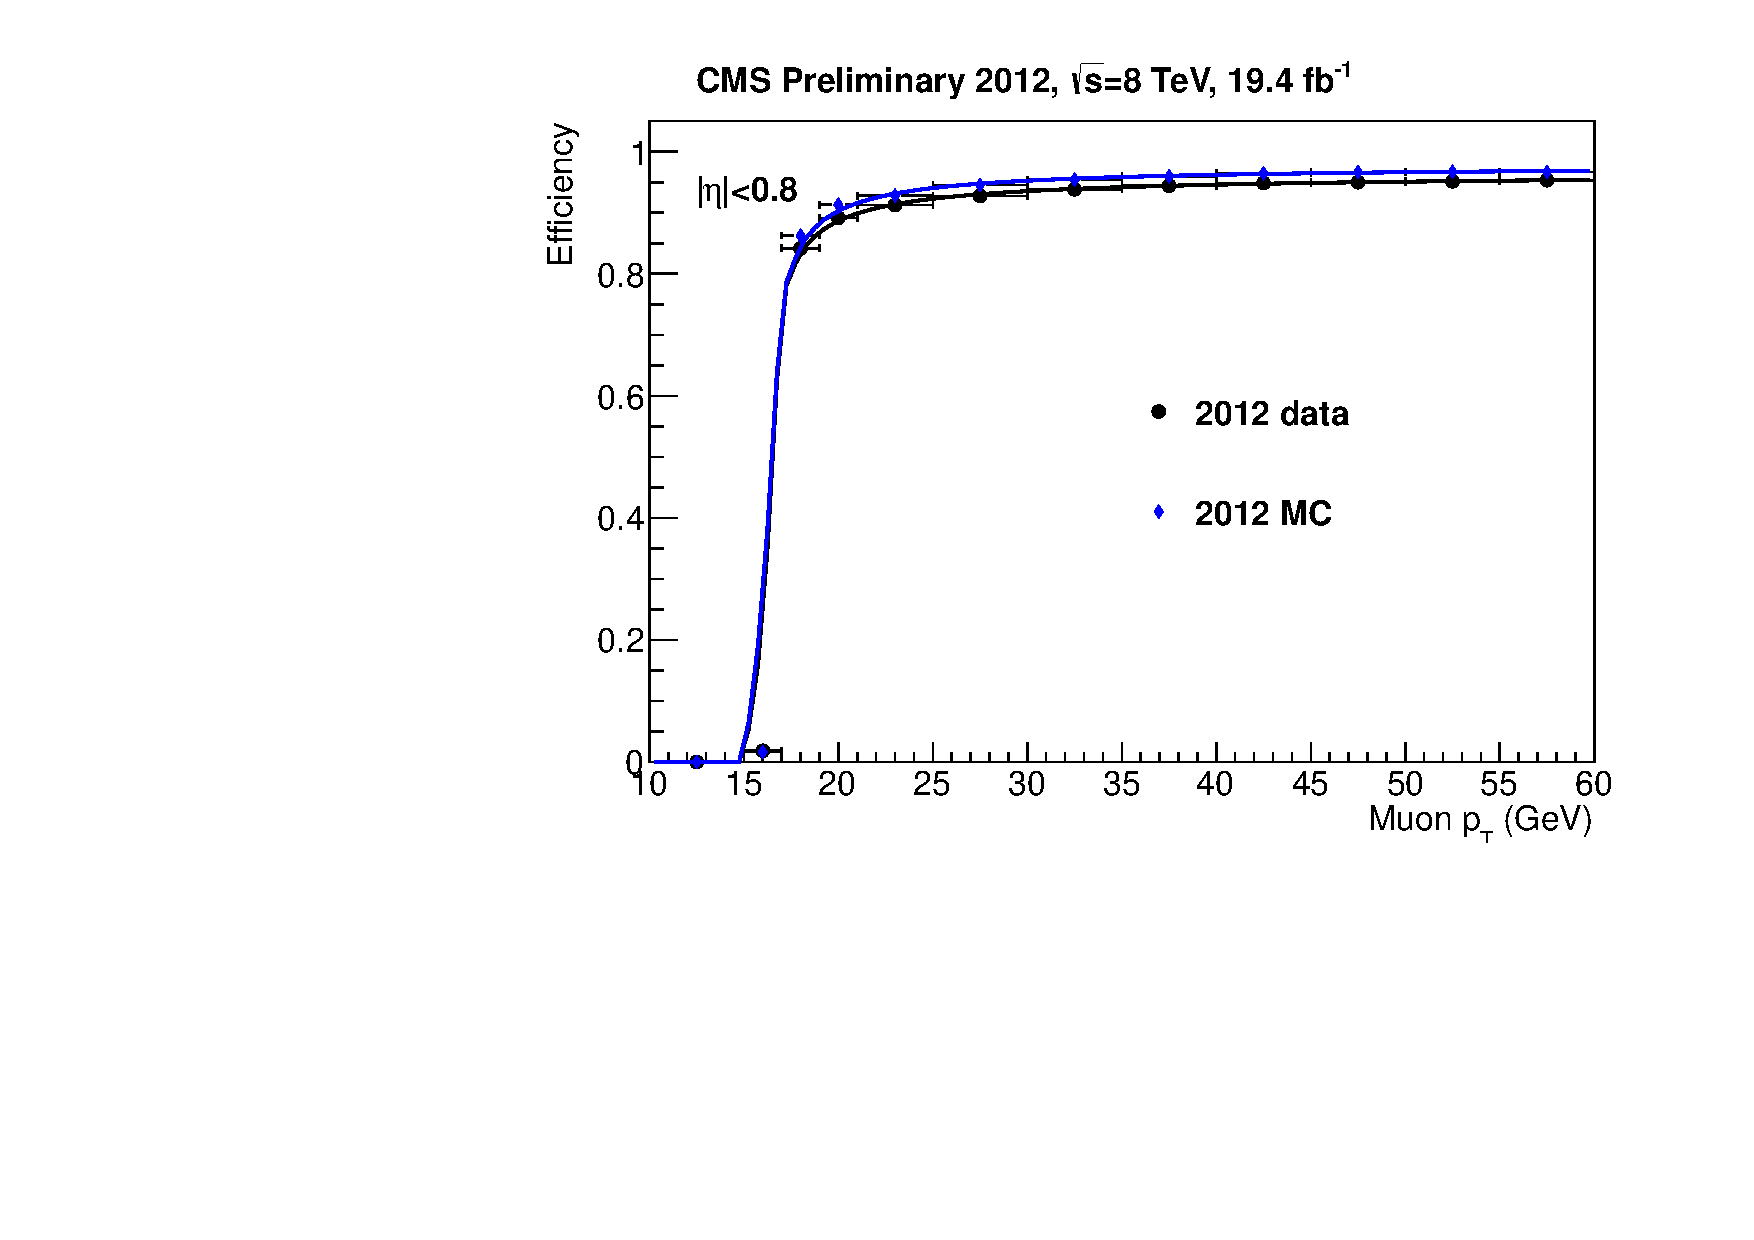
\includegraphics[width=0.5\textwidth]{plots/TagAndProbe/MuonAbsEta082012DatavsMC.pdf}
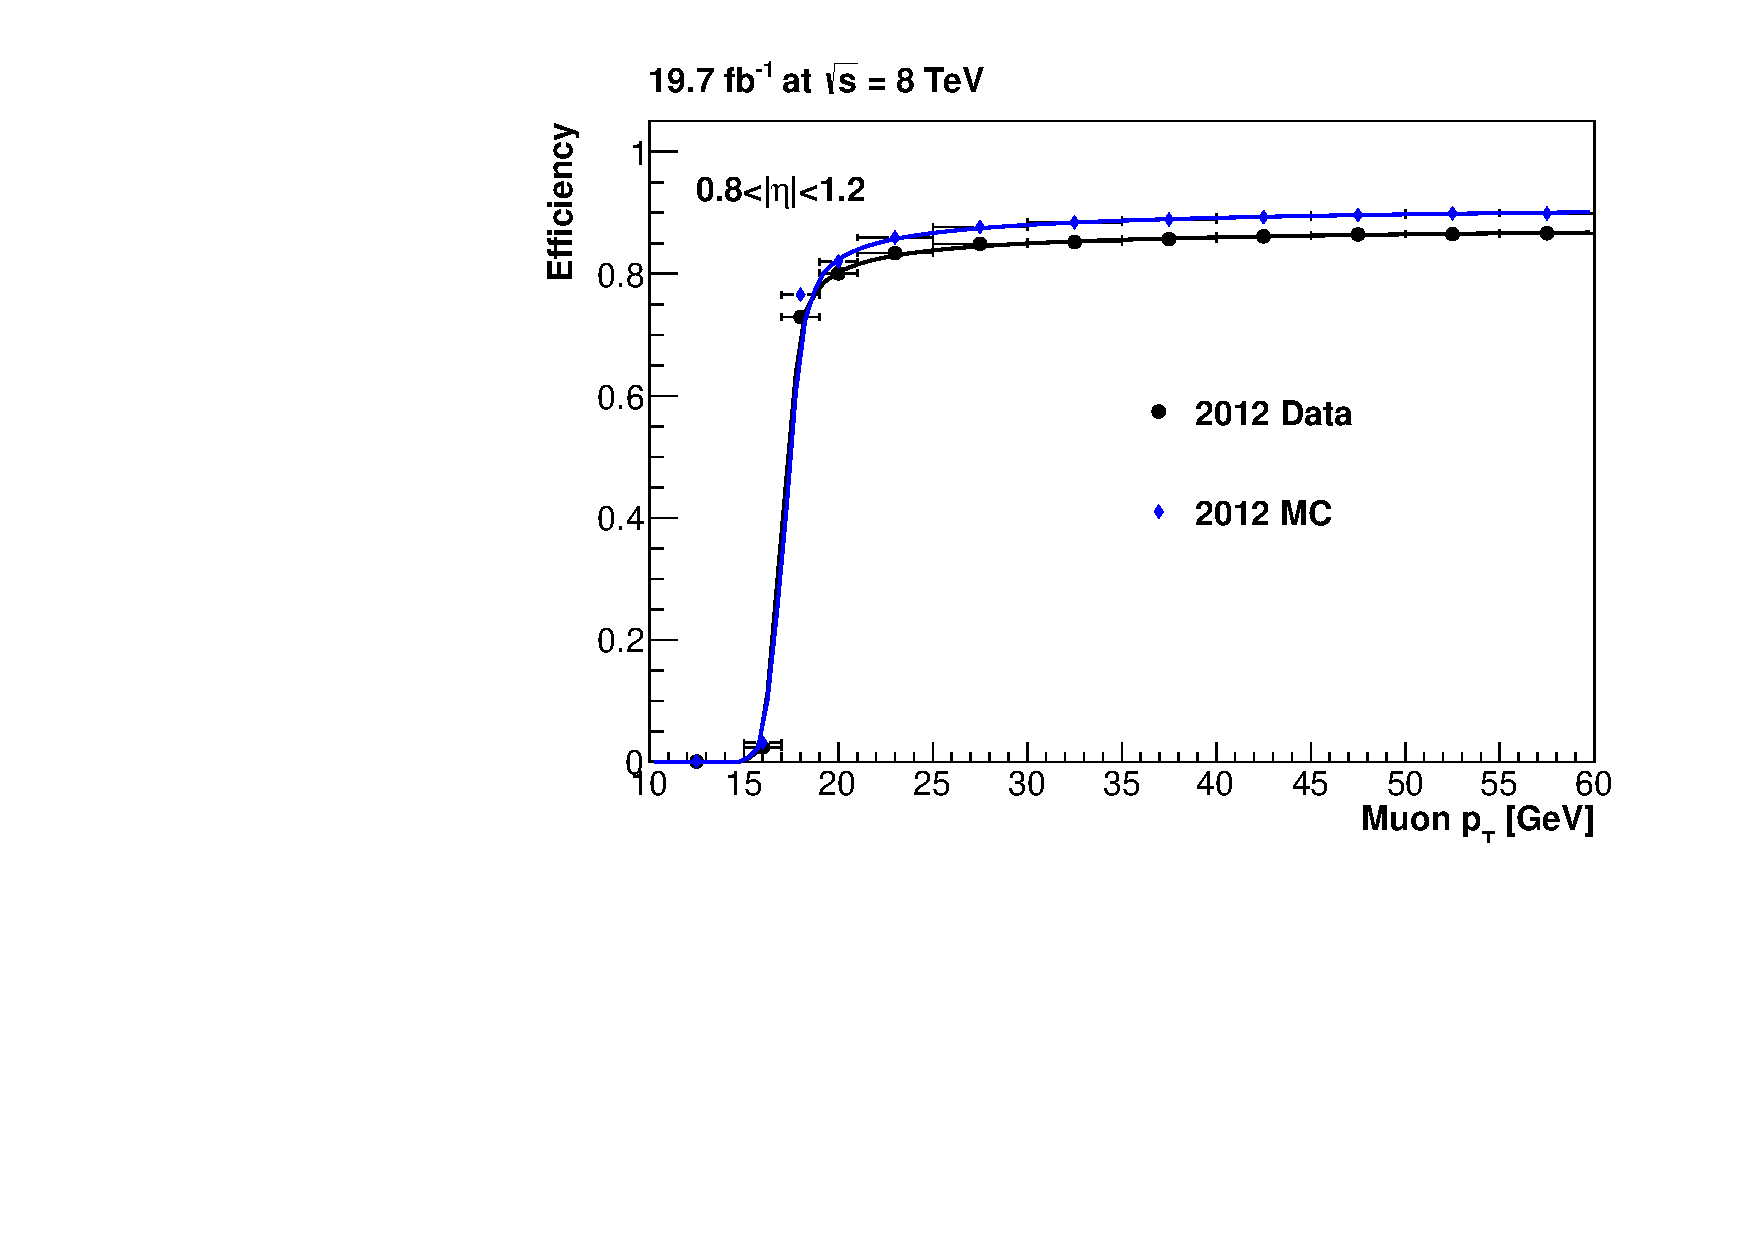
\includegraphics[width=0.5\textwidth]{plots/TagAndProbe/MuonAbsEta122012DatavsMC.pdf}
\begin{center}
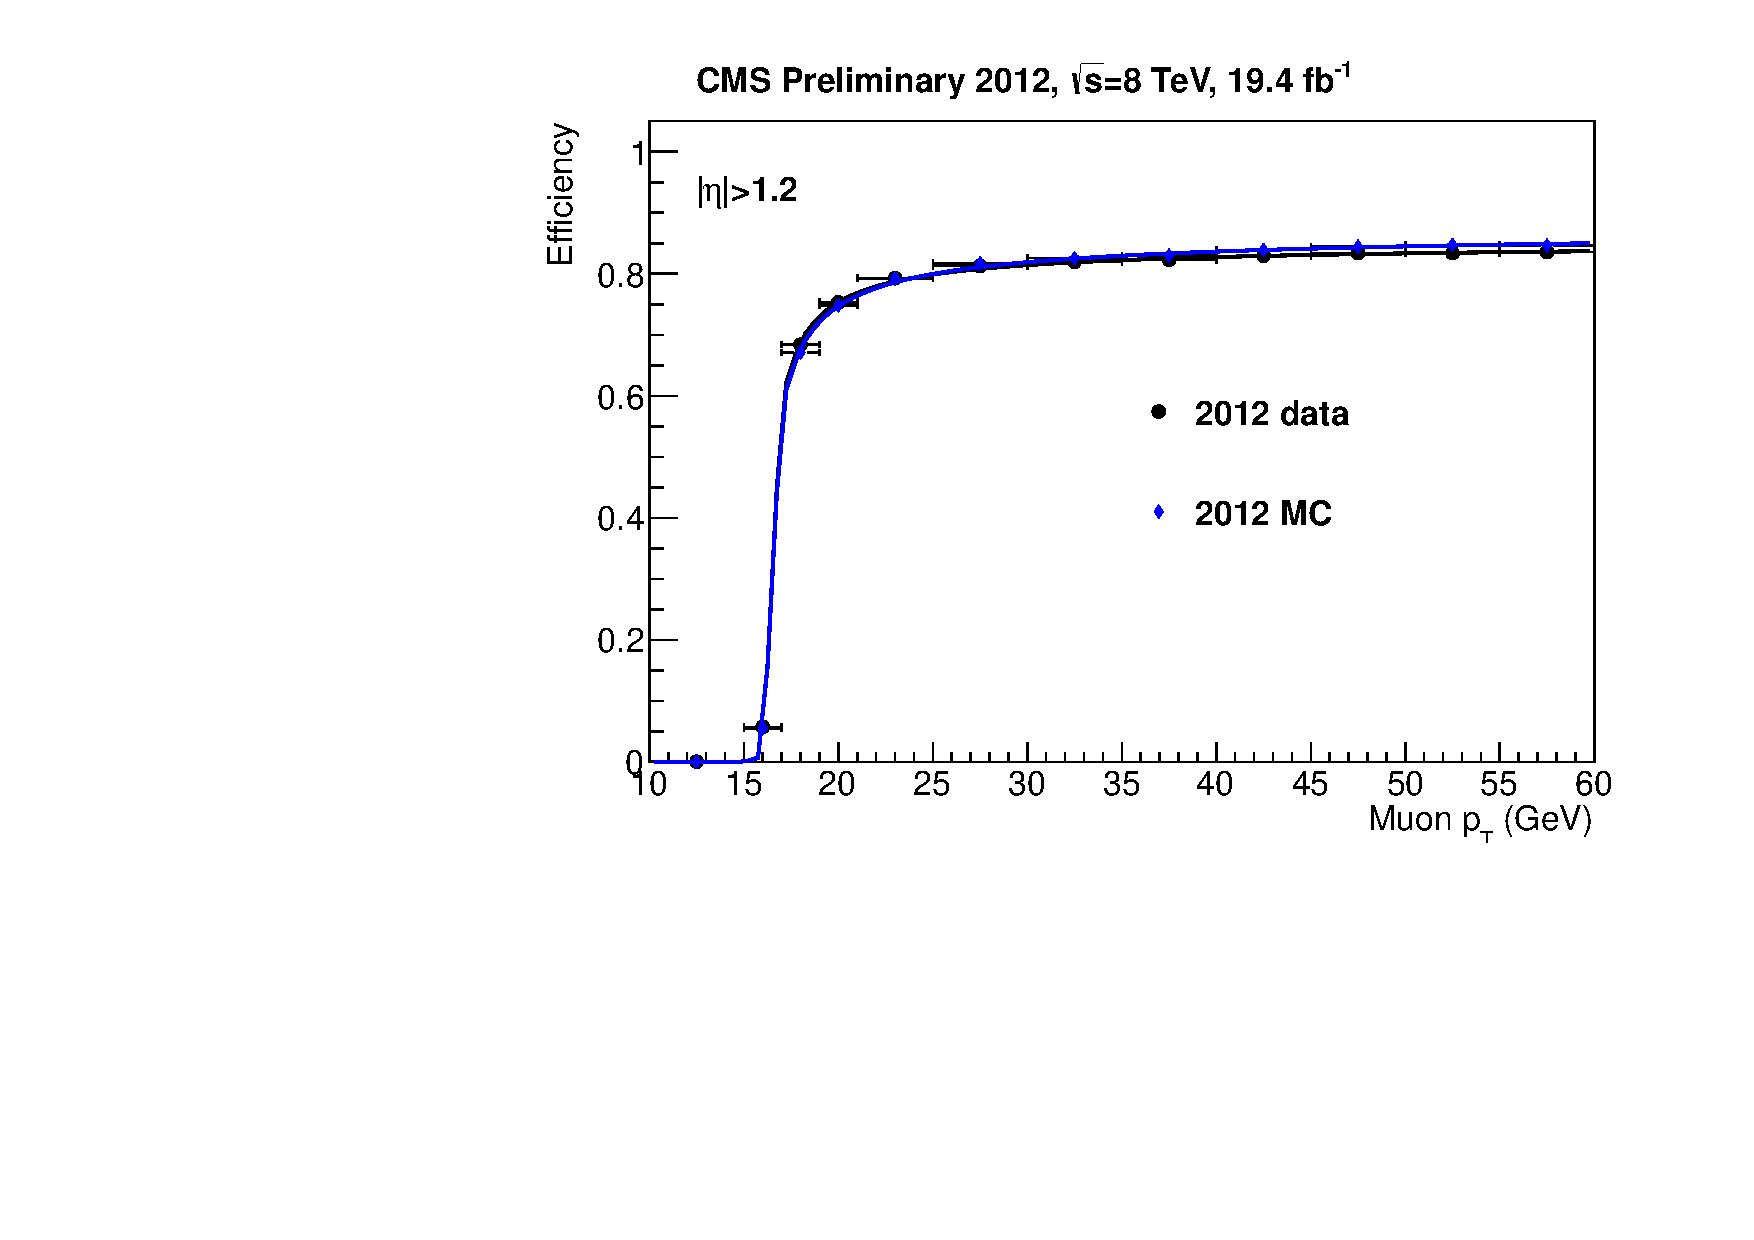
\includegraphics[width=0.5\textwidth]{plots/TagAndProbe/MuonAbsEndcap2012DatavsMC.pdf}
\end{center}
\caption{Trigger efficiency as a function of muon p$_{\rm{T}}$ measured in
2012 data and MC in the region (top left) $|\eta|$ $<$ 0.8, (top right) 0.8
$<$ $|\eta|$ $<$ 1.2 and (bottom) $|\eta|$ $>$ 1.2.}
\label{fig:muontrg}
\end{figure}


\section{Control Plots}

\section{Results}

Plan for layout:
-Introduction
-Objects/triggers (refers back to previous chapters)
-Background estimation-->mostly data driven but point out where MC is needed -->
tag and probe, few pages.
-categories
-svfit?
-control plots (pre fit)
-systematics (brief)

Interpretation (maybe separate chapter)
-fit and pulls
-limit and significance
-Other important statistical results
